\section{Gruppeteori}
\begin{frame}{Gruppeteori}
\begin{itemize}
	\item<1-> Gruppe definition 
	\begin{itemize}
		\item<1->  $(set,operator)$ 
	\end{itemize}
	\item<1-> Rubik's gruppen
	\begin{itemize}
		\item<1-> $M_1 * M_2 \in G$ 
		\item Tomt move: $e*M=M$
		\item Invers move: $M$ og $M'$
		\item Associative lov: $(M_1 * M_2) * M_3 = M_1 * (M_2 * M_3)$
	\end{itemize}
\end{itemize}
\end{frame}

\begin{frame}{Gruppeteori}
\begin{itemize}
	\item Undergruppe
	\begin{itemize}
		\item H-gruppen
		\begin{itemize}
			\item Alle cubies har korrekt orientation
			\item Cubies i midterlag
			\item Lukket under: ``U, U', U2, D, D', D2, R2, L2, F2, B2''
		\end{itemize}
	\end{itemize}
\end{itemize}

\only<1>{
\begin{figure}
	\centering
		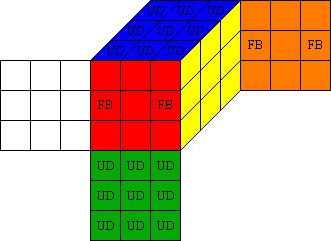
\includegraphics[width=0.6\textwidth]{../../rapport/input/pics/relabelClean.PNG}
	\label{fig:sdf}
\end{figure}}

\only<2>{
\begin{figure}
	\centering
		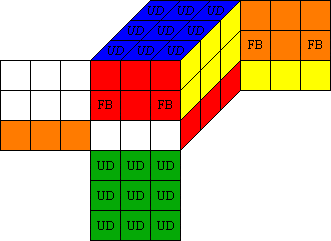
\includegraphics[width=0.6\textwidth]{../../rapport/input/pics/relabelD.PNG}
	\label{fig:sdf2}
\end{figure}}

\only<3>{
\begin{figure}
	\centering
		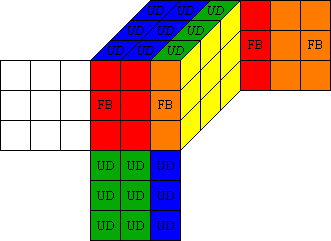
\includegraphics[width=0.6\textwidth]{../../rapport/input/pics/relabelR2.PNG}
	\label{fig:sdf3}
\end{figure}}


\end{frame}